% Idea 5 contribution: one analysis section, one paragraph for the shared Discussion,
% an appendix block (not graded), and the AI-disclosure text.
% Needs graphicx and booktabs. Cites rezaei2025egonormia (already in the team .bib as Rezaei et al., 2025; adjust the key).
% Rename "Analysis 2" if the team assigns a different slot.

%%%%%%%%%%%%%%%%%%%% MAIN TEXT %%%%%%%%%%%%%%%%%%%%
\section{Analysis 2: Is Spatial Evidence Present, and Can a Frozen Model Use It?}

\paragraph{Motivation and hypotheses.} Idea 5 proposes giving the model explicit geometry and body/hand pose for social-norm reasoning. That rests on two premises we can check without training: that spatial reasoning is actually what EgoNormia items ask for, and that geometric maps carry something a model does not already extract from RGB. We test \textbf{H1}, spatial content is concentrated in a subset of norm categories rather than spread across the benchmark; \textbf{H2}, a contextual language representation separates spatially defined (Proxemics) items better than interpretable lexical ones; and \textbf{H3}, appending pose, segmentation, or depth maps changes a frozen VLM's answers beyond extra-image and mismatched-map controls.

\paragraph{Data and protocol.} \emph{Language (H1, H2).} We use the answer text of all 1{,}853 EgoNormia items \citep{rezaei2025egonormia} from 1{,}075 source videos, concatenating each action with its justification (7{,}412 options). We compare mean-pooled \texttt{bert-base-uncased} embeddings with two interpretable representations: Empath's 194 lexical categories, and a fixed list of spatial terms (e.g.\ \emph{distance, space, behind, aside}) and body terms (e.g.\ \emph{hand, gesture, facing}) written before inspecting results. Probes are logistic regressions with five folds grouped by source video; intervals are 95\% item bootstraps. \emph{Vision (H3).} On 40 items from distinct source videos, chosen by a fixed hash before any inference, we sample five pre-action frames and derive body/hand pose (MediaPipe), instance segmentation (YOLOv8n-seg), and relative depth (Depth Anything V2). Frozen models answer from RGB alone or RGB plus maps, with two controls: the RGB grid repeated, and maps taken from a different video. The metric requires action and justification both correct. No weights are updated.

\paragraph{Results.} \emph{H1.} A spatial term appears in 24.6\% of correct options overall. It is most frequent for Privacy (40.0\%) and Proxemics (33.7\%) and least for Cooperation (20.9\%; Figure~\ref{fig:idea5-spatial}); the Empath categories most over-represented in Proxemics options are \emph{movement} (23\% vs.\ 14\%) and \emph{body} (15\% vs.\ 10\%). \emph{H2.} Predicting whether Proxemics is among an option's labels gives AUC 0.67 with BERT, against 0.58 for Empath and 0.59 for the two-feature lexicon; a six-way probe on the primary category reaches 45.7\% [43.5, 48.0] with BERT and 34.7\% [32.5, 36.9] with Empath (majority 25.8\%). A t-SNE of the embeddings shows overlapping regions rather than clusters (Appendix). Consistent with the TF-IDF probe in Analysis~1, a BERT probe over option text alone selects the correct option on 58.6\% [56.3, 60.8] of items (chance 25\%). \emph{H3.} Added maps do not improve any model (Table~\ref{tab:idea5-frozen}). For Qwen3-VL-8B, aligned pose scores 15/40 against 16/40 for RGB, and pose from an unrelated video also scores 15/40; repeating the RGB grid moves more answers (5 of 40) than adding pose (2 of 40). Claude gives the identical answer in all 16 input conditions on 14 of 15 items; the single item that changes also changes under the repeated-RGB and mismatched-map controls. A GPT-5.6 agent is correct on 11/15 items from RGB, and none of its four failures is recovered by any map or description. Extractor coverage is limited: a body or hand is returned in 81 of 200 frames (40.5\%), and segmentation produces evident class errors (\emph{horse}, \emph{bird} on a construction site).

\begin{figure}[t]
\centering
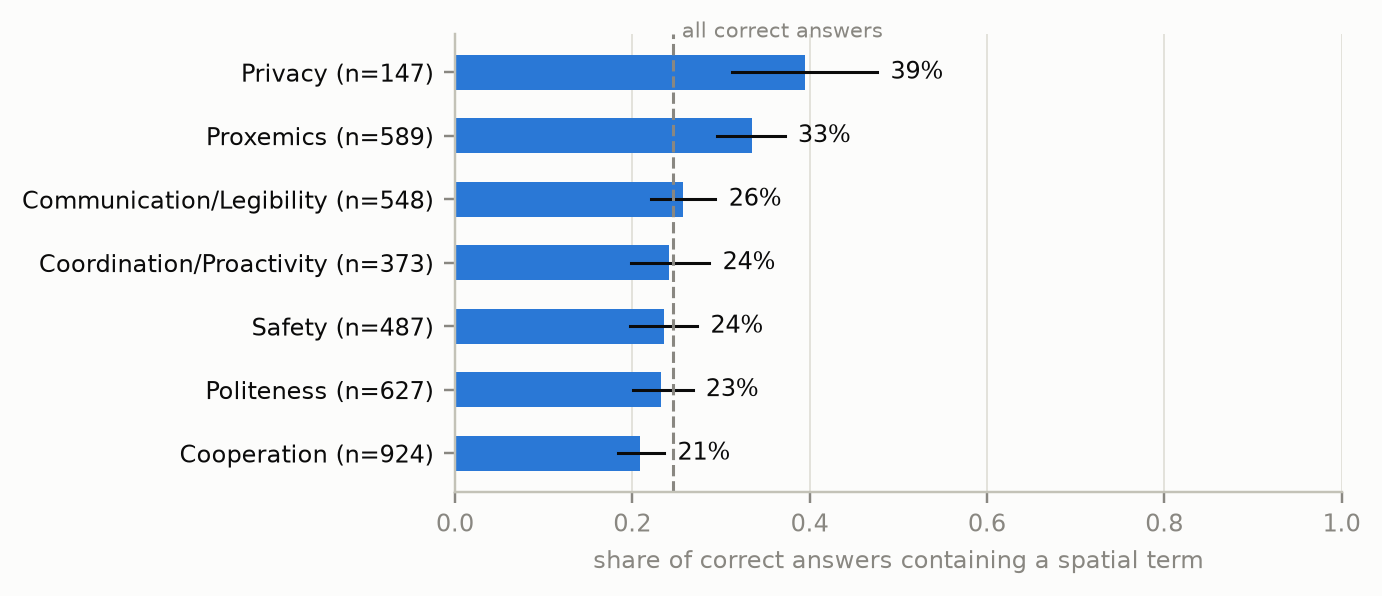
\includegraphics[width=\linewidth]{spatial_language.png}
\caption{Share of correct answer options containing at least one spatial term, by norm category (an option can carry several categories). Bars show 95\% bootstrap intervals; the dashed line is the rate over all correct options.}
\label{fig:idea5-spatial}
\end{figure}

\begin{table}[t]
\caption{Joint accuracy (action and justification both correct) of frozen models with geometry maps appended to RGB. ``+all'' adds pose, segmentation and depth; ``+repeat'' repeats the RGB grid; ``+mism.'' uses maps from a different video. Qwen3-VL-8B was run with pose only.}
\label{tab:idea5-frozen}
\centering\small
\setlength{\tabcolsep}{3pt}
\begin{tabular}{lrrrrr}
\toprule
Model & RGB & +pose & +all & +repeat & +mism. \\
\midrule
Qwen3-VL-8B ($n{=}40$) & 16 & 15 & -- & 13 & 15 \\
%QWEN32B_ROW
Claude Opus 5.5 ($n{=}15$) & 12 & 12 & 13 & 13 & 13 \\
\bottomrule
\end{tabular}
\end{table}

\paragraph{Qualitative check.} Two of the 15 items are answered incorrectly by both GPT-5.6 and Claude in every input condition (a clothing-store scene and a construction-site scene). In the clothing-store item the depth map does show a companion close to the camera wearer, and the model notes this, but it does not change the chosen action: the map confirms what the RGB frames already show.

\paragraph{Discussion of Analysis 2.} The premises of Idea 5 hold only in part. Spatial content exists but is a minority signal: three in four correct answers use no spatial vocabulary, and it concentrates in Proxemics and Privacy. Bolting geometry onto a frozen model does nothing measurable, and the mismatched-map control shows why: the models are not reading the maps, so there is no alignment-dependent effect to find. Because the maps are derived from the same RGB frames, they add a re-encoding rather than new information, and they are empty in most frames of egocentric video where the wearer's body is out of view. These are small samples (15--40 items) and agent-based runs for GPT and Claude, so they establish the absence of an immediate benefit, not that adaptation would fail.

%%%%%%%%%%%%%%%%%%%% FOR THE SHARED DISCUSSION SECTION %%%%%%%%%%%%%%%%%%%%
\paragraph{Implications for Idea 5.} We keep the idea but change how it is tested. First, geometry will be evaluated on the Proxemics and Privacy subsets, reported separately from overall accuracy, since that is where spatial content concentrates and where an effect, if any, should appear. Second, every geometry result will be reported against three controls established here: a text-only probe (which already selects 58.6\% of answers), a repeated-RGB input, and mismatched maps. Without the last two, a change caused by an extra image slot would be mistaken for a geometry effect. Third, appending rendered maps at inference is dropped as a method; the model must be adapted to the representation, and we will carry a missing-detection indicator rather than a blank image, since pose is absent in about 60\% of frames. Fourth, we will replace the COCO-class segmenter, whose label errors inject wrong information, and prioritise hand pose and depth, the two signals that remain available in egocentric views. EgoNormia items used here were scored against labels, so they are excluded from training and from future model selection.

%%%%%%%%%%%%%%%%%%%% APPENDIX (not graded) %%%%%%%%%%%%%%%%%%%%
% \section{Analysis 2: Supplementary Results}
% \paragraph{Representations.} Figure~\ref{fig:idea5-probe} compares the three language representations; Figure~\ref{fig:idea5-tsne} shows the t-SNE. Choosing the longest option gives 21.7\%; correct and distractor options average 22.0 and 22.8 words, so length is not the cue.
% \paragraph{Frozen-model conditions.} Sixteen conditions: RGB, +pose, +segmentation, +depth, +all three, RGB repeated once, RGB repeated three times, and all maps from another video, each with and without generated text descriptions of every image. Claude joint accuracy over 15 items, images / with descriptions: RGB 12/12, pose 12/12, segmentation 13/12, depth 13/13, all 13/12, repeat once 13/12, repeat three times 13/13, mismatched 13/12. Each condition was answered by a separate agent with no access to labels or to other conditions.
% \paragraph{Pose availability.} Body output in 59/200 frames, hand output in 36/200, either in 81/200, both in 14/200; 31 of 40 clips have an output in at least one frame. These are detector-output counts, not validated accuracy.
% \begin{figure}[h]\centering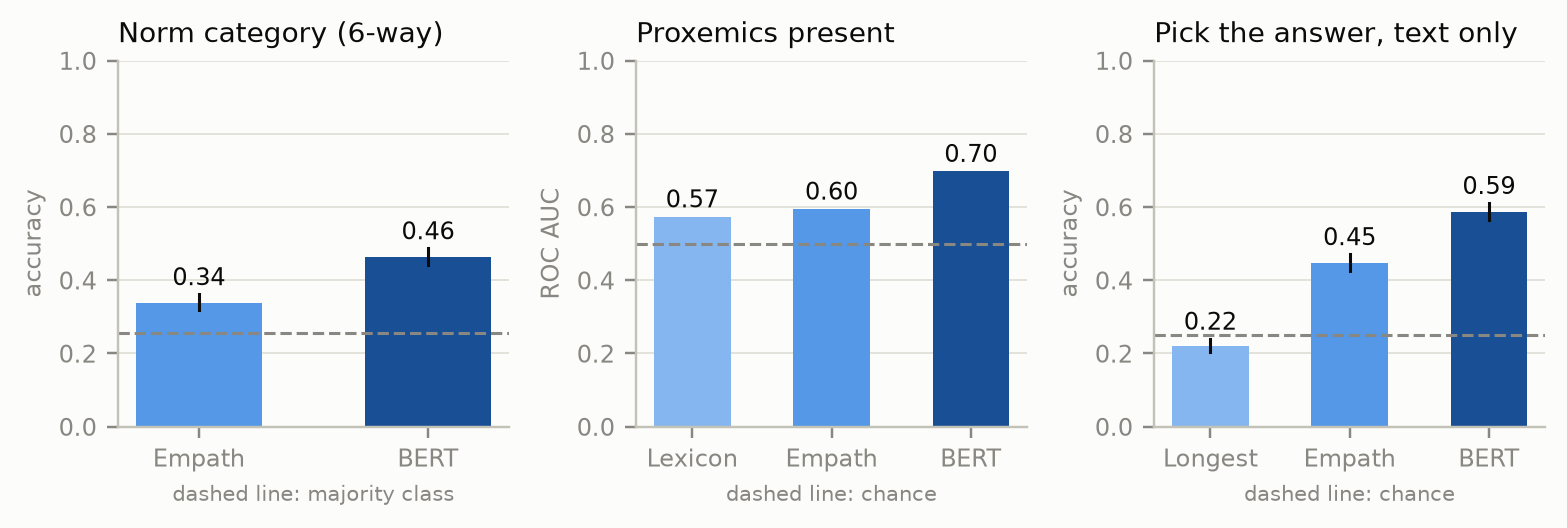
\includegraphics[width=\linewidth]{representation_comparison.png}
% \caption{Language representations compared on three label-related questions; folds grouped by source video.}\label{fig:idea5-probe}\end{figure}
% \begin{figure}[h]\centering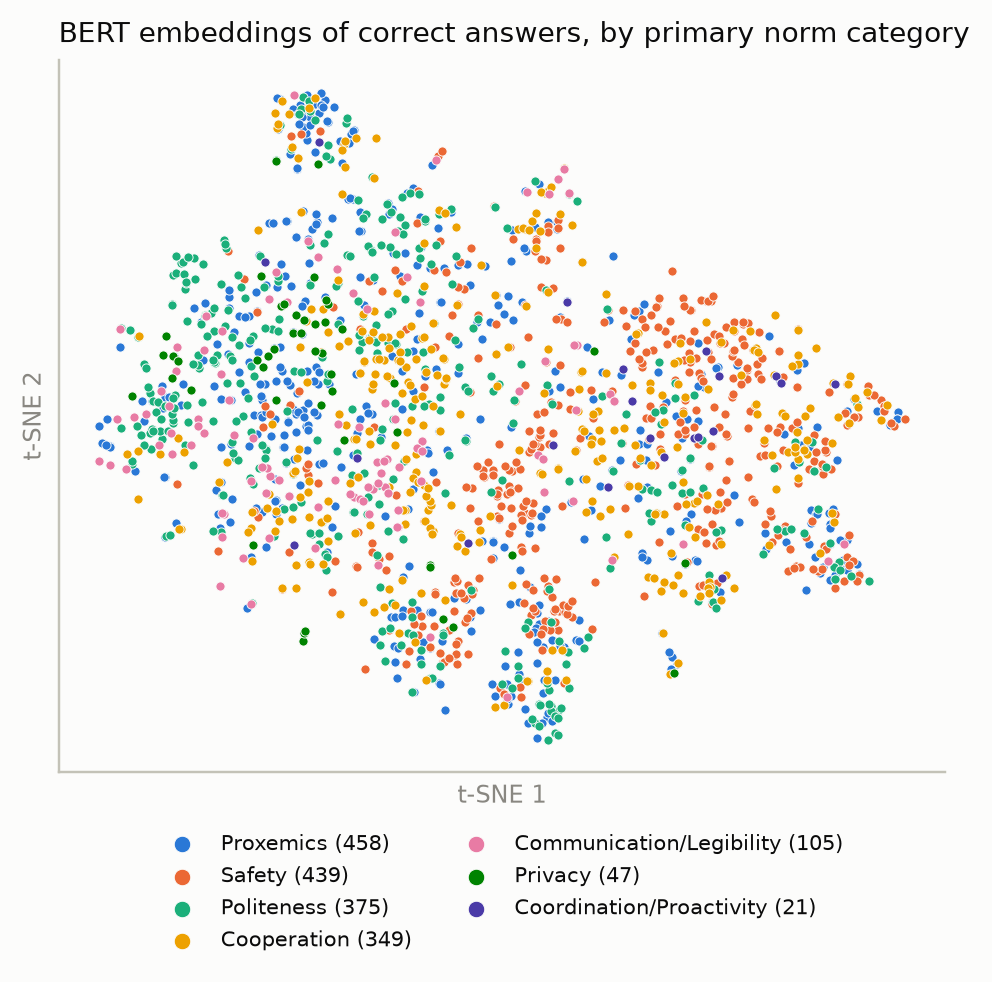
\includegraphics[width=0.8\linewidth]{tsne_category.png}
% \caption{t-SNE of BERT embeddings of correct options, coloured by primary norm category.}\label{fig:idea5-tsne}\end{figure}

%%%%%%%%%%%%%%%%%%%% AI DISCLOSURE (edit to match what you did) %%%%%%%%%%%%%%%%%%%%
% Analysis 2: OpenAI Codex downloaded EgoNormia, selected the fixed 40-item sample, wrote and ran the pose,
% segmentation and depth extraction and the Qwen3-VL inference, and spawned a GPT-5.6 agent that answered
% items from images. Claude (Claude Code) ran the same items through Claude Opus 5.5 agents, wrote and ran the
% language analysis (BERT, Empath, lexicon), produced the figures, and drafted this section and the
% Idea 5 discussion paragraph. Models used as tools: Qwen3-VL-8B/32B, MediaPipe, YOLOv8n-seg,
% Depth Anything V2, bert-base-uncased, Empath. Shiv Gupta chose the analyses, directed the experiments,
% and reviewed the results and text. [State here what you inspected and rewrote yourself.]
